\section{Experiments and Analysis}

In this section, we first assess the reliability of the proposed benchmark metrics and their alignment with human preference.
We then train different interactive world modeling approaches on WildWorld and evaluate them on WildBench using the ground truth annotations provided in WildWorld dataset.

\subsection{Compared Approaches}

\noindent
\textbf{Camera-Conditioned Video Generation}.
In this setting, model takes a camera trajectory, an initial image, and a text prompt as inputs to generate a video that follows the defined camera motion.
We fine-tune the Wan2.2-Fun-5B-Control-Camera~\cite{wan2025wan} model with camera trajectories ground-truth in WildWorld dataset, the resulting model is dubbed as \textit{\textbf{CamCtrl}}.
The baseline model uses a rule-based approach to convert discrete camera control action inputs into
camera poses, from which it computes Plücker embeddings~\cite{plkemb} for each frame and injects them into
the model.
In contrast, we directly use the ground-truth per-frame camera poses in WildWorld as inputs for fine-tuning.

\noindent
\textbf{Skeleton-Conditioned Video Generation}.
Skeletal pose provides a direct and fine-grained representation of character motion.
We introduce a skeleton-conditioned setting that takes the first frame and a skeleton video as inputs.
We fine-tune Wan2.2-Fun-5B-Control~\cite{wan2025wan}, a video-to-video model that supports skeleton-based pose videos as a control signal, and dub the resulting model \textbf{\textit{SkelCtrl}}.
To construct the skeleton video, we use the per-frame 3D skeleton keypoints and their joint-tree structure annotated in the WildWorld dataset, project them into screen coordinate under the ground-truth camera pose, and render them as a colored-skeleton video matching the input format expected by the baseline model. \par\nopagebreak[4]

\noindent
\textbf{State-Conditioned Video Generation}.
Based on \textit{\textbf{CamCtrl}}, we design a state-aware model: \textit{\textbf{StateCtrl}}, which injects states into the video generation process.
We first perform structured modeling of different states, dividing them into discrete states (\textit{e.g.}, monster type, weapon category) and continuous states (\textit{e.g.}, coordinates, health).
Discrete states are mapped to vector representations through trainable embedding, while continuous states are encoded into the same feature space using an MLP.
At the encoding stage, we adopt a hierarchical modeling strategy with entity-level and global-level representations.
Each entity (\textit{e.g.}, monster) encodes its own states, while global states (such as recording time) are also incorporated.
We use transformer \cite{vaswani2017attention} architecture to model the relationships between entities, producing a unified state embedding representation.
The resulting embedding is aligned with video frames and injected into the intermediate layers of DiT as a conditioning signal to guide the video generation process.
In addition, we introduce a state decoder to recover the state information from the state embedding representation, a state predictor to predict the next-frame state.
During training, a decoder loss is used to ensure that the embedding preserves the original states;
a predictor loss is used to supervise the state predictor, enhancing the temporal consistency and predictability of the state representation.
During inference, \textit{\textbf{StateCtrl}} supports using only the ground-truth state of the first frame, while the states of subsequent frames are autoregressively predicted by the state predictor.
We denote this model as \textbf{\textit{StateCtrl-AR}}.

\noindent
Across all settings, models are trained at a resolution of $544 \times 960$ with 81 frames per sample and a frame rate of 16 FPS, using a batch size of 1 and a learning rate of $1\times10^{-5}$.
Training is performed for 250,000 iterations with a batch size of 8 using the Adam optimizer.
During inference, we adopt the same resolution and frame rate, and use 50 sampling steps.

\begin{table*}[t]
\centering
\renewcommand{\arraystretch}{1.3}
\setlength{\tabcolsep}{5.0pt}
\caption{Comparison of different interactive video generation approaches trained on WildWorld and evaluated on WildBench. Lower is better for ATE and RPE; higher is better for the others.}
\begin{tabular}{l|cccc|cc|c|c}
\hline
\multirow{2}{*}{Method} 
& \multicolumn{4}{c|}{Video Quality} 
& \multicolumn{2}{c|}{Camera Control} 
& \multicolumn{1}{c|}{Action} 
& \multicolumn{1}{c}{State} \\
\cline{2-5}\cline{6-7}
& MS 
& DD 
& AQ 
& IQ
& ATE($\downarrow$)
& RPE($\downarrow$)
& \multicolumn{1}{c|}{Following}
& \multicolumn{1}{c}{Alignment} \\
\hline
Baseline & 96.38 & 99.00 & 50.81 & 65.62 & 4.63 & 0.18 & 53.77 & 11.29 \\
CamCtrl & 97.85 & 97.00 & 48.29 & 62.88 & 2.02 & 0.13 & 83.46 & 15.18 \\
SkelCtrl & 97.85 & 95.00 & 47.92 & 62.43 & 2.55 & 0.10 & 92.81 & 22.03 \\
StateCtrl & 97.45 & 99.00 & 50.86 & 67.78 & 0.94 & 0.07 & 85.66 & 16.06 \\
StateCtrl-AR & 97.43 & 99.00 & 50.90 & 67.76 & 1.01 & 0.08 & 74.66 & 16.13 \\
\hline
\end{tabular}
\label{tab:main_results}
\end{table*}


\subsection{Overall Evaluation}

\noindent
\textbf{Evaluation of the Proposed Benchmark Metrics}.
We validate the reliability of the proposed Action Following and State Alignment metrics, as well as their alignment with human preference.
For Action Following, we use the same evaluation protocol with human judgments instead of model-based assessment. 
Specifically, 10 volunteers are recruited, and each segment is annotated by three volunteers.
Segments with inconsistent annotations are discarded, accounting for about 5\% of the full set. 
We then measure the consistency between human judgments and model scores.
For State Alignment, we run keypoint tracking directly on ground truth videos and evaluate the resulting trajectories using the same protocol to verify the reliability of the metric.

The experimental results show that human judgments and the proposed model-based Action Following metric achieve 85\% agreement on WildBench, indicating that the metric can reliably reflect human evaluation of action consistency.
Moreover, the State Alignment metric achieves 43.23\% coordinate accuracy against the  skeleton ground-truth, demonstrating its effectiveness in measuring alignment between generated and ground-truth state evolution.

\noindent
\textbf{Evaluation of the Interactive Video Generation}. Table~\ref{tab:main_results} presents the WildBench evaluation results of different interactive world model approaches trained on the WildWorld dataset. Here, Baseline refers to Wan2.2-TI2V-5B~\cite{wan2025wan}, and Video Quality is reported as a percentage. We observe that

\begin{itemize}
    \item \textbf{All approaches improve over the baseline on interaction-related metrics}.
    For example, the camera-conditioned video generation model \textit{\textbf{CamCtrl}} reduces ATE and RPE on Camera Control by $\triangle$2.61 and $\triangle$0.05, respectively. 
    Taking skeletal video as conditional input, \textit{\textbf{SkelCtrl}} achieves nearly 100\% average improvement on Action Following and State Alignment.
    Moreover, directly conditioning on discrete and continuous state information, \textit{\textbf{StateCtrl}} and \textit{\textbf{StateCtrl-AR}} improve performance across all three metrics.
    This highlights the usefulness of our WildWorld dataset, as diverse approaches can benefit from it.

    \item \textbf{VBench appear saturated on WildWorld.} We observe that all methods achieve over 95\% on the MS (Motion Smoothness) and DD (Dynamic Degree) metrics under Video Quality.
    In contrast, their actual ability to produce reasonable motion and dynamics still differs substantially, as evidenced by the large performance difference on Action Following and State Alignment.
    This suggests that interactive world models require more fine-grained and nuanced evaluation metrics to assess highly dynamic video generation, which aligns with the design goal of WildBench.
    
    \item \textbf{Directly using visual signals as conditional input yield a trade-off.}
    We find that \textit{\textbf{SkelCtrl}}, which uses visual signals for interactive control input, achieves larger gains on interaction-related metrics than \textit{\textbf{StateCtrl}}, which learns soft embeddings from the same information; however, it comes at the cost of lower video quality, as reflected by decreased AQ (Aesthetic Quality) and IQ (Image Quality) scores under the Video Quality evaluation. We further analyze this pattern in the qualitative evaluation blow.

    \item \textbf{Autoregressive interactive world models show promise}.
    Using only the first-frame state and autoregressively predicting subsequent states as control inputs, \textit{\textbf{StateCtrl-AR}} achieves performance comparable to \textit{\textbf{StateCtrl}}, but exhibits a noticeable drop in \textbf{Action Following}.
    We attribute this degradation to error accumulation in iterative next-state prediction, a phenomenon also observed in autoregressive video generation~\cite{huang2025self,longlive,ji2025memflow}.
    We believe this paradigm can be combined with autoregressive video generation and may even further advance its development.

\end{itemize}

\begin{figure*}[t]
\centering
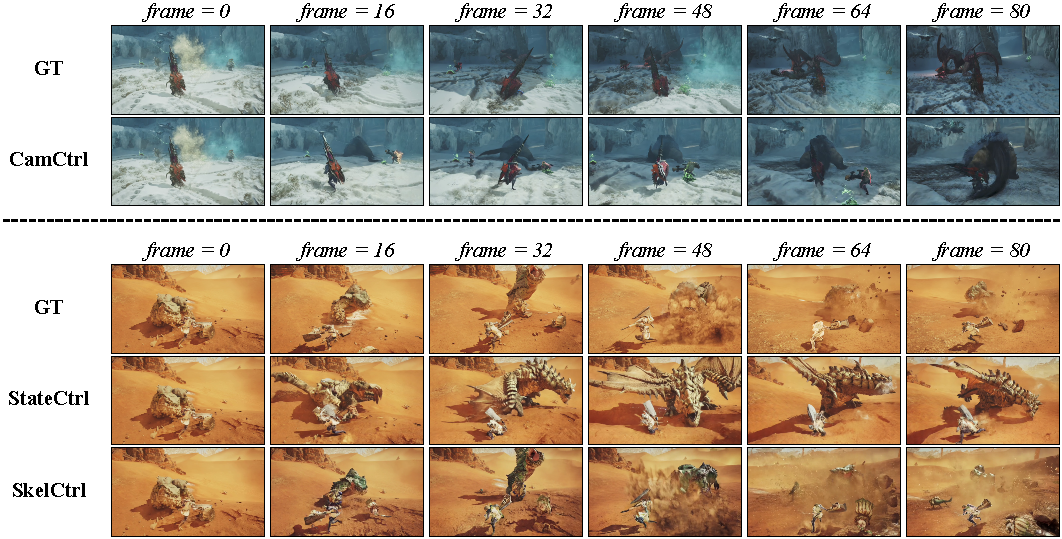
\includegraphics[width=\linewidth]{figures/qualitative_comparison_v2.pdf}
\caption{Qualitative comparisons of different interactive world modeling approaches trained on the WildWorld dataset.}
\label{fig:visualization}
\end{figure*}

\subsection{Qualitative Evaluation}

Table~\ref{fig:visualization} presents visual comparisons of different interactive world modeling approaches on two test examples.
The top example shows that \textit{\textbf{CamCtrl}} produces camera motion consistent with the ground truth, but fails to capture the monster’s dynamics.
In particular, for the bottom example, we observe that \textit{\textbf{StateCtrl}} generates a clearer foreground subject, whereas in the ground truth the subject is partially occluded by splashing sand and gravel; in contrast, \textit{\textbf{SkelCtrl}} better reproduces this effect. This observation is consistent with the abovementioned stronger image-quality performance of \textit{\textbf{StateCtrl}}, as clearer frames are typically perceived as having higher image quality.
